\documentclass[]{standalone}

\usepackage{../lenses}

\begin{document}
 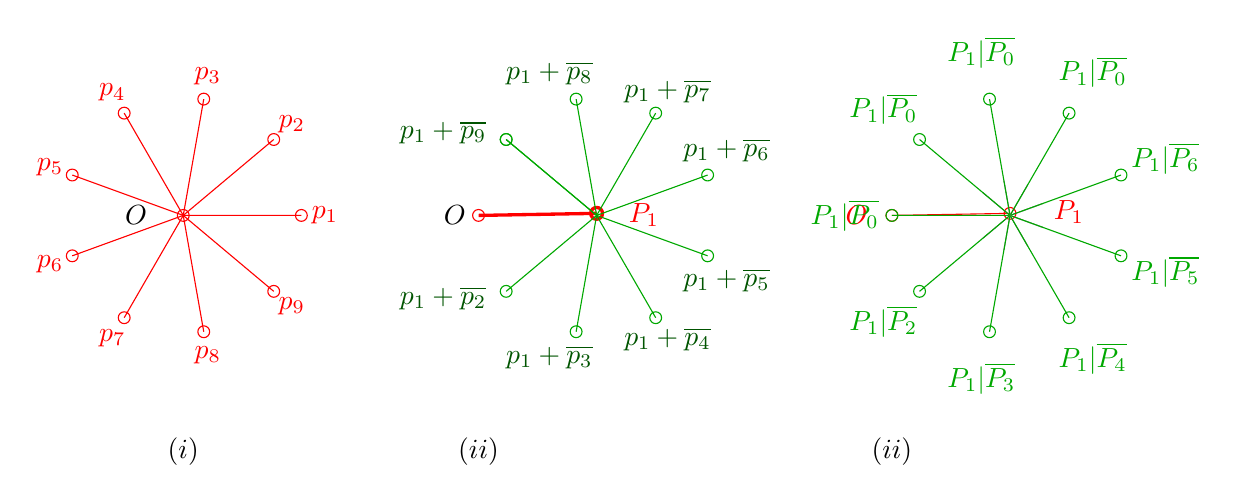
\begin{tikzpicture}
  \begin{scope}[scale=1.5]
  
   \begin{scope}[shift={(0,0)}]
    \draw[red](0,0) circle(0.05);
    \foreach \x in {1,2,3,4,5,6,7,8,9} {
     \pgfmathsetmacro{\n}{40*(\x-1)}
     \draw[red](0,0) -- (\n:1) circle(0.05) ++(\n:0.2) node{$p_\x$};
    }
    \draw(-0.4,+0.0) node{$O$};
    \path(0,-2) node{$(i)$};
   \end{scope}

   \begin{scope}[shift={(2.5,0)}]
    \draw[red](0,0) circle(0.05);
    \draw[red,very thick](0,0) -- (1:1) circle(0.05);
    \begin{scope}[shift={(1,0)}]
     \foreach \x in {0,2,3,4,5,6,7,8,9} {
      \ifthenelse{\x=0}{ } {
       \pgfmathsetmacro{\n}{180+40*(\x-1)}
       \draw[green!66!black](0,0) -- (\n:1) circle(0.05);
      }
     }
     \draw(-1.2,+0.0) node{$O$};
     \draw(+0.4,+0.0) node[red]{$P_1$};
     \draw(+1.1,+0.55) node[green!33!black]{$p_1+\overline{p_6}$};
     \draw(+1.1,-0.55) node[green!33!black]{$p_1+\overline{p_5}$};
     \draw(+0.6,+1.05) node[green!33!black]{$p_1+\overline{p_7}$};
     \draw(+0.6,-1.05) node[green!33!black]{$p_1+\overline{p_4}$};
     \draw(-0.4,+1.2) node[green!33!black]{$p_1+\overline{p_8}$};
     \draw(-0.4,-1.2) node[green!33!black]{$p_1+\overline{p_3}$};
     \draw(-1.3,+0.7) node[green!33!black]{$p_1+\overline{p_9}$};
     \draw(-1.3,-0.7) node[green!33!black]{$p_1+\overline{p_2}$};
    \end{scope}
    \path(0,-2) node{$(ii)$};
   \end{scope}

   \begin{scope}[shift={(6,0)}]
    \draw[red](0,0) circle(0.05) ++(-0.3,0.0) node{$O$};
    \draw[red](0,0) -- (1:1) circle(0.05) ++(1:0.5) node{$P_1$};
    \begin{scope}[shift={(1,0)}]
     \foreach \x [count=\c] in {0,2,3,4,5,6,0,0,0} {
      \pgfmathsetmacro{\n}{180+40*(\c-1)}
      \ifthenelse{\x=0}{ 
       \draw[gray](0,0) -- (\n:0.3);
      } {
       \draw[green!66!black](0,0) -- (\n:1) circle(0.05) ++(\n:0.4) node[]{$P_1|\overline{P_\x}$};
      }
     }
    \end{scope}
    \path(0,-2) node{$(ii)$};
   \end{scope}


  \end{scope}
 \end{tikzpicture}
\end{document}